% don't remove the folling lines, and edit the defintion of \main if needed
\documentclass[../report.tex]{subfiles}
\providecommand{\main}{..}
\IfEq{\jobname}{\currfilebase}{\AtEndDocument{\biblio}}{}
% until here

\begin{document}

\newcommand{\gl}{\ensuremath{\tilde{g}}}
\newcommand{\tone}{\ensuremath{\tilde{t}_1}}
\newcommand{\neut}{\ensuremath{\tilde{\chi}}}
\newcommand{\stopq}{\ensuremath{\tilde{t}}}
\newcommand{\chiOneZero}{\ensuremath{\tilde{\chi}_1^0}}
\newcommand{\chiTwoZero}{\ensuremath{\tilde{\chi}_2^0}}
\newcommand{\chiOnePM}{\ensuremath{\tilde{\chi}_1^\pm}}
\newcommand{\chiOneMP}{\ensuremath{\tilde{\chi}_1^\mp}}
\newcommand{\Ptmiss}{\ensuremath{p_T^{miss}}}
\newcommand{\Dmstop}{\ensuremath{\Delta m(\stopq,\chiOneZero)}}

\section{Supersymmetry}
\label{sec:BSM-SUSY}

Supersymmetry (SUSY) remains the only known dynamical solution to the Higgs naturalness problem that can be extrapolated up to very high energies, in a consistent and calculable way. It gives a successful framework for gauge coupling unification; it automatically predicts a potential candidate for DM; it turns the Higgs mass into a calculable parameter; it gives a conceptual justification for EWSB; it offers a hint for a final reconciliation between gravity and gauge forces. In spite of this impressive list of attractive features, there is no firm experimental evidence that speaks in favour of SUSY. The results from the LHC have already constrained significantly a variety of models that implement SUSY at the EW scale and have contributed to shift the focus of the continuing experimental scrutiny. The questions that need to be answered are whether SUSY can still be the key to understand Higgs naturalness but its implementation at the EW scale is less simple than originally assumed, or whether SUSY is the key to understanding EWSB but its implementation comes at the price of some amount of tuning. Both these questions can only be answered by further experimental investigation. The most important targets to gather information about these questions are the SUSY particles that directly affect the Higgs mass and thus contribute more sizeably to the degree of tuning. These are the top squarks (stops) and the Higgsinos. Moreover, because of an accidentally large two-loop contribution to the stop mass, the gluino also plays a central role in the degree of naturalness of SUSY models. Nonetheless, the interest in understanding the full structure of the theory strongly motivates also the search for the other SUSY particles (squarks, sleptons, and EW gauginos), especially since the limits from the LHC on sleptons and EW gauginos are still rather weak in comparison to those on strongly interacting particles.   

SUSY may be realised in nature in a variety of different models, leading to distinct collider signals coming from production of superpartners. Coloured SUSY particles such as squarks and gluinos are produced via the strong interaction and have the highest cross-sections at hadron colliders. EW gauginos and Higgsinos mix into neutralino and chargino mass states, which will be collectively referred to as electroweakinos (EWkinos). Their production cross-sections depend on mixing parameters and are typically much smaller than those of coloured superpartners at hadron colliders. 
For this reason, the EW sector remains more difficult to test at hadron machines and searches at $e^{+}e^{-}$ colliders would complement the SUSY parameter space coverage. The null results from searches at the LHC motivate scrutiny of less conventional as well as more experimentally difficult processes where SUSY may lurk. These include the cases of nearly-degenerate mass spectra, non-prompt decays and exotic signatures.

\subsection{Gluinos and squarks} 
The expected reach of gluino (\gl) searches at hadron colliders is shown in Fig.~\ref{fig:SUSY_gluino}, for $R$-parity conserving scenarios and under simplifying assumptions on the $\gl$ prompt decay mode.  In all cases, the lightest neutralino ($\tilde \chi_1^0$) is assumed to be the lightest supersymmetric particle (LSP). Exclusion limits at 95\% CL are presented; the corresponding definitive observation with a significance of $5\sigma$ is 5--10\% lower for each process. The most stringent gluino bounds are found for massless LSP. If the gluino is close in mass to the LSP, the topology is referred to as `compressed' and the amount of missing transverse momentum (\Ptmiss) in the event decreases. The typical multijet + \Ptmiss~SUSY searches are less effective and must be replaced with monojet-like analyses, where the gluinos recoil against an initial state radiation (ISR) jet. Lepton colliders are ineffective in the search for gluinos, which are neutral with respect to the EW interaction.

%\begin{figure}[t]
\begin{figure}[htb]
    \centering
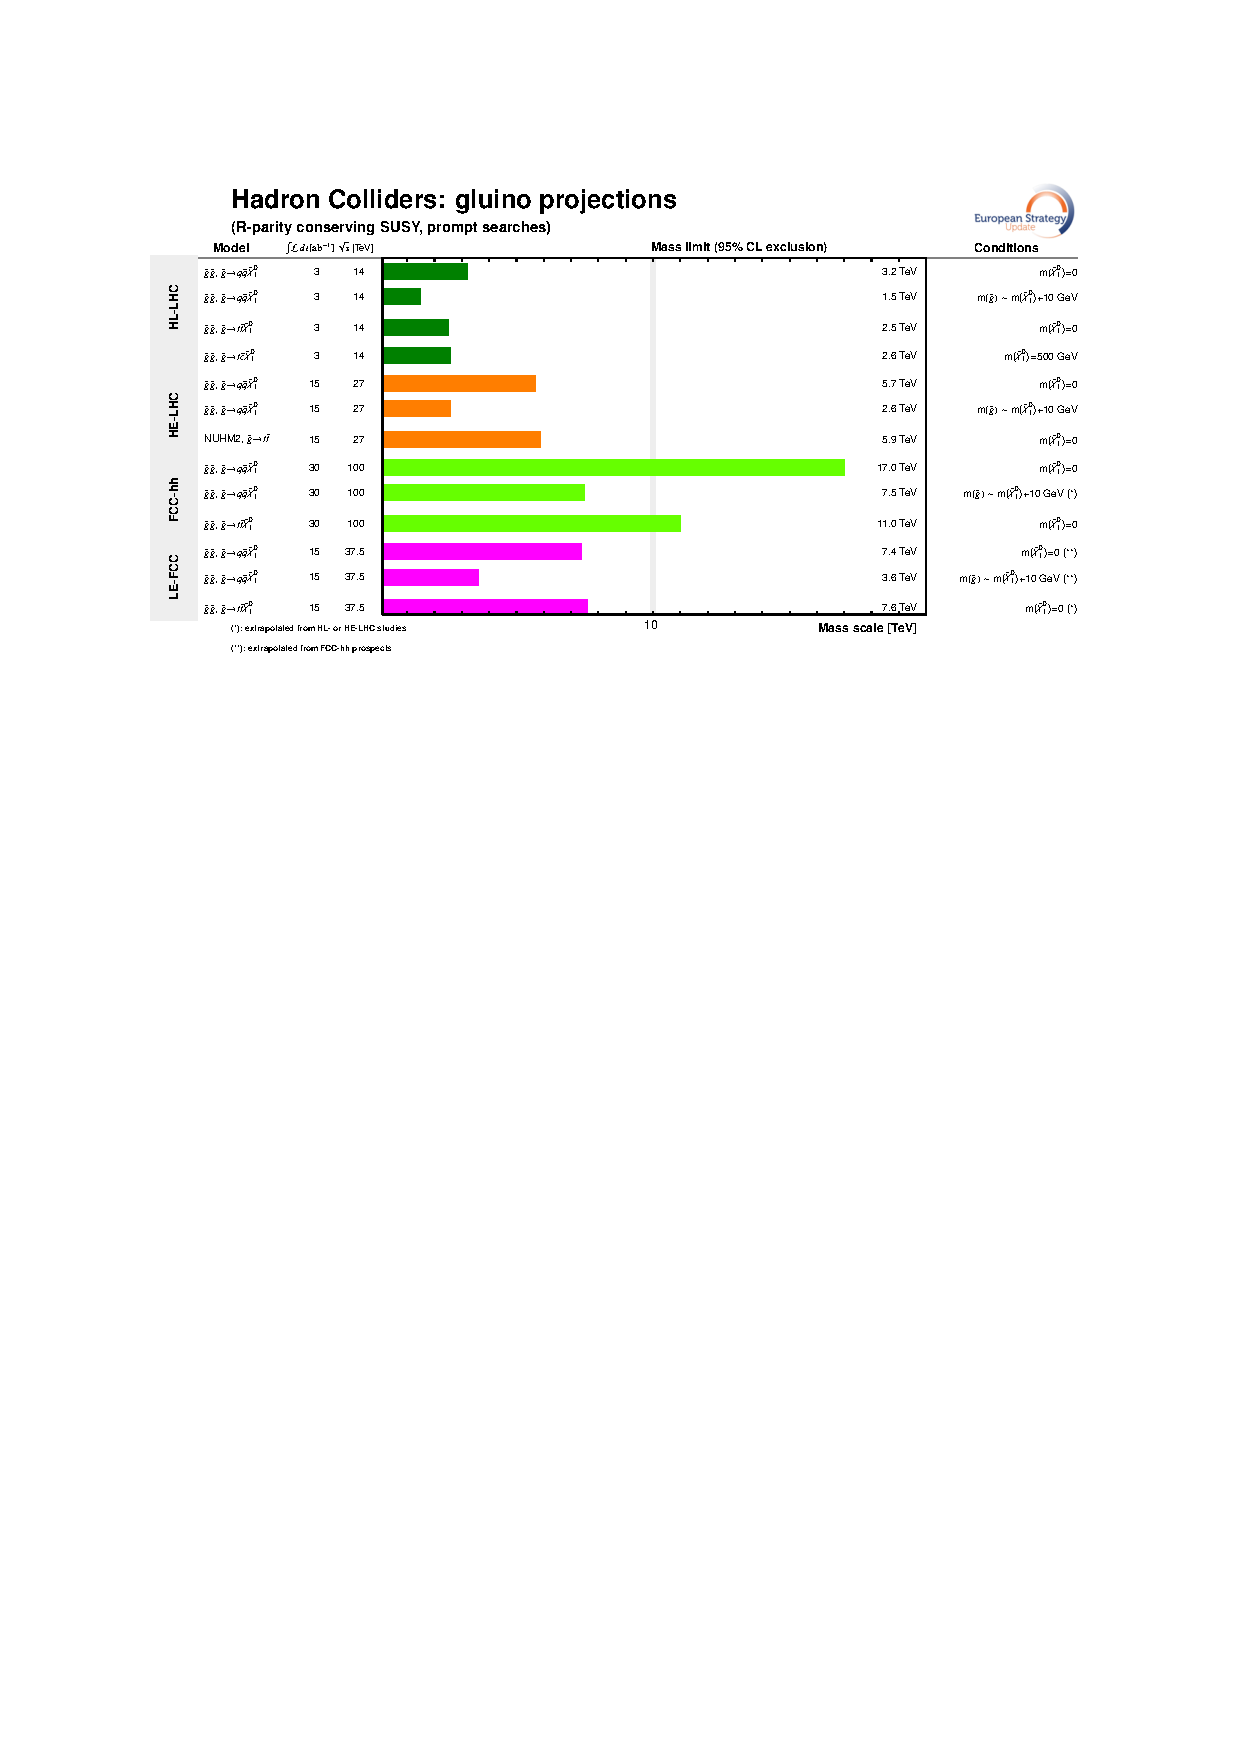
\includegraphics[width=1.0\textwidth]{\main/BSM/SUSY/plots_SUSY/AllCollider-Gluino-LEFCC-cropped.pdf}
%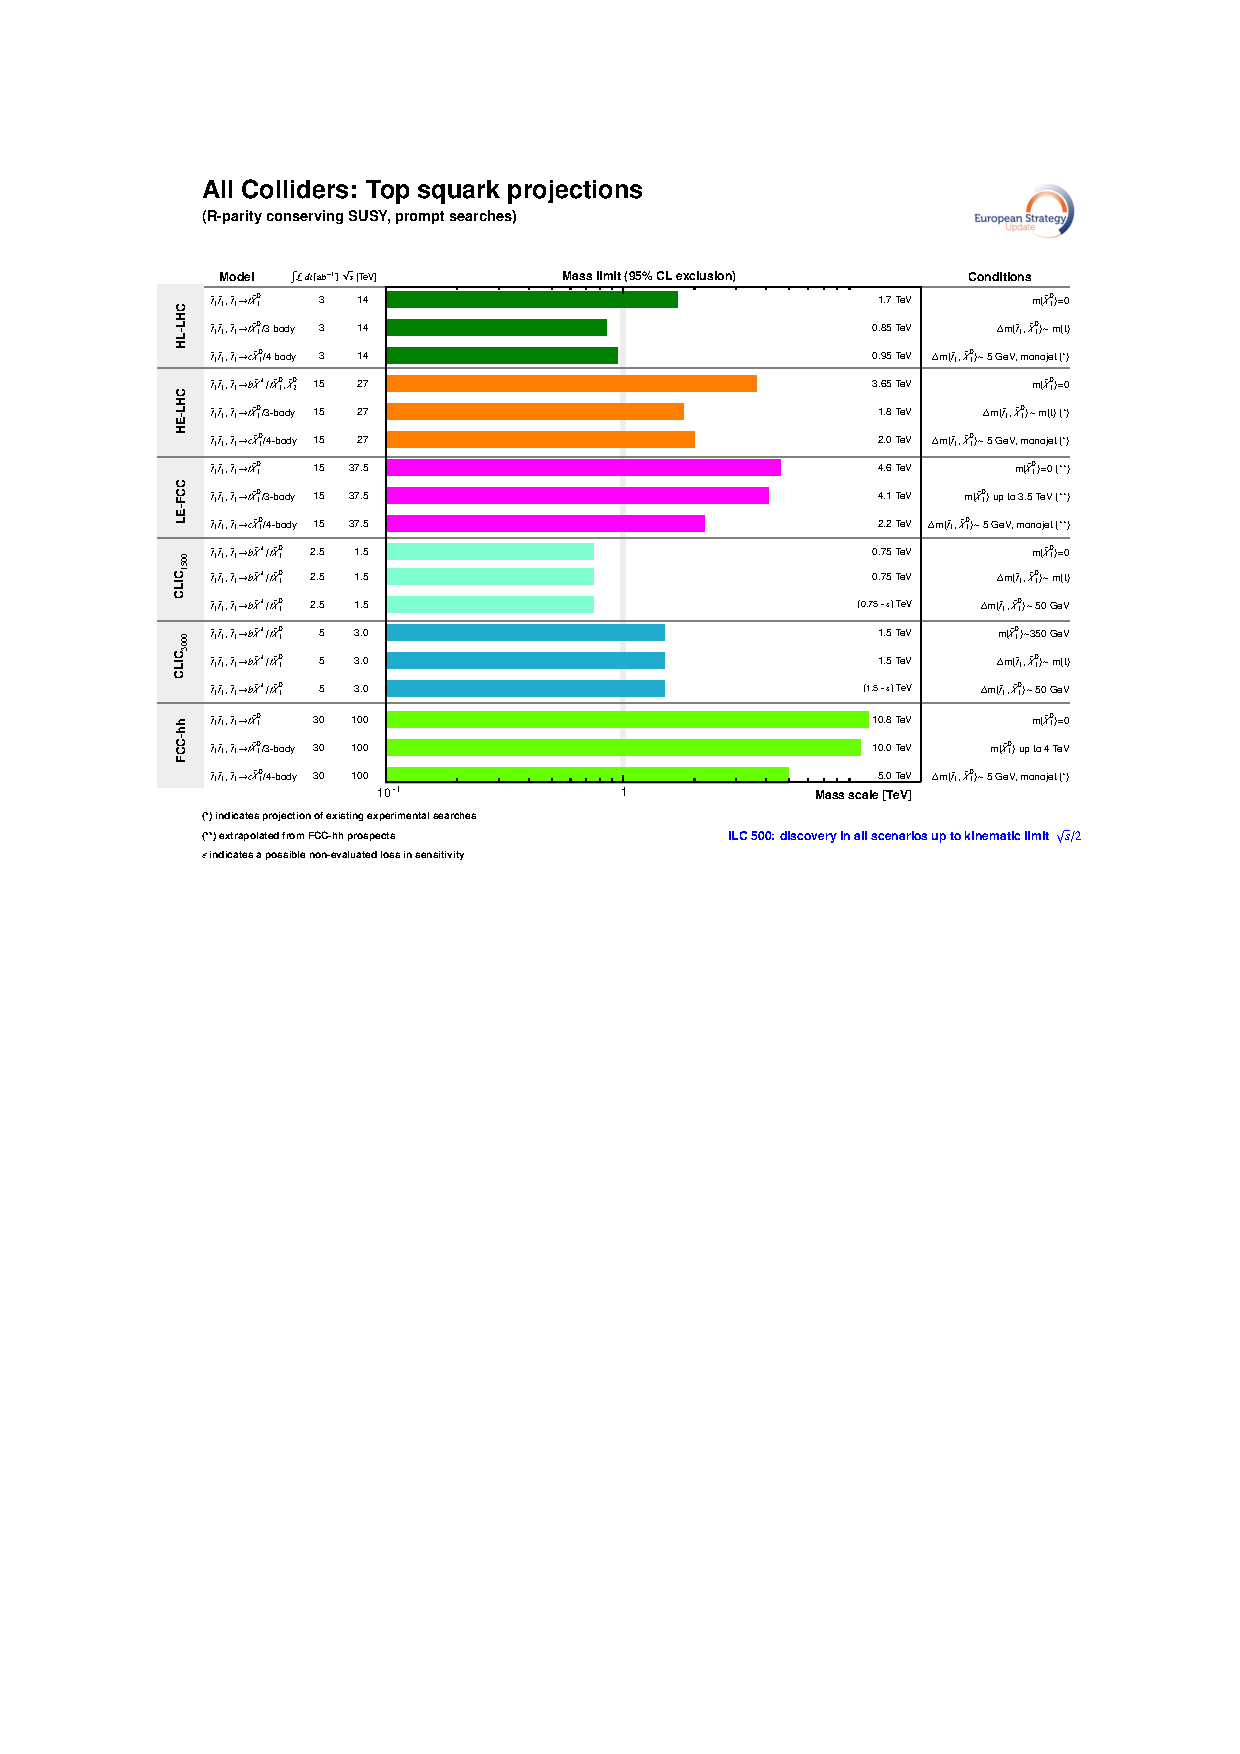
\includegraphics[width=0.45\textwidth]{\main/BSM/SUSY/plots_SUSY/AllCollider-Stop-LEFCC.pdf}
    \caption{
    %\emph{Left:} 
    Gluino exclusion reach of different hadron colliders: HL- and HE-LHC~\cite{CidVidal:2018eel}, and FCC-hh~\cite{Golling:2016gvc, Abada:2019lih}. Results for low-energy \FCChh is obtained with a simple extrapolation.
    %\emph{Right:} Exclusion reach for top squarks for hadron and lepton colliders. In both cases, the reach of a Low-Energy FCC option is also shown.}
    }
\label{fig:SUSY_gluino}
\end{figure}

While there are no recent projections on searches for first- and second-generation squarks at \HLLHC~\cite{ATL-PHYS-PUB-2014-010} and \HELHC, the 95\% CL exclusion reach for models where squarks decay directly into a quark and a neutralino can be extrapolated from the recent ATLAS and CMS results using Run 2 data (36~fb$^{-1}$, see for example ref.~\cite{PhysRevD.97.112001} and~\cite{Khachatryan2017}). Two scenarios and analysis approaches are considered: massless neutralino (from jets+\Ptmiss~searches) and mass splitting of 5~GeV between the squark and neutralino (inferred from monojet searches). The results are shown in Fig.~\ref{fig:SUSY_squarks}. Extrapolated prospects for the LE-FCC are also reported, as well as the reach for \CLICThreeThousand (private communication) and results of dedicated studies at the \FCChh~\cite{Golling:2016gvc}.

\begin{figure}[htb]
%\begin{figure}[t]
    \centering
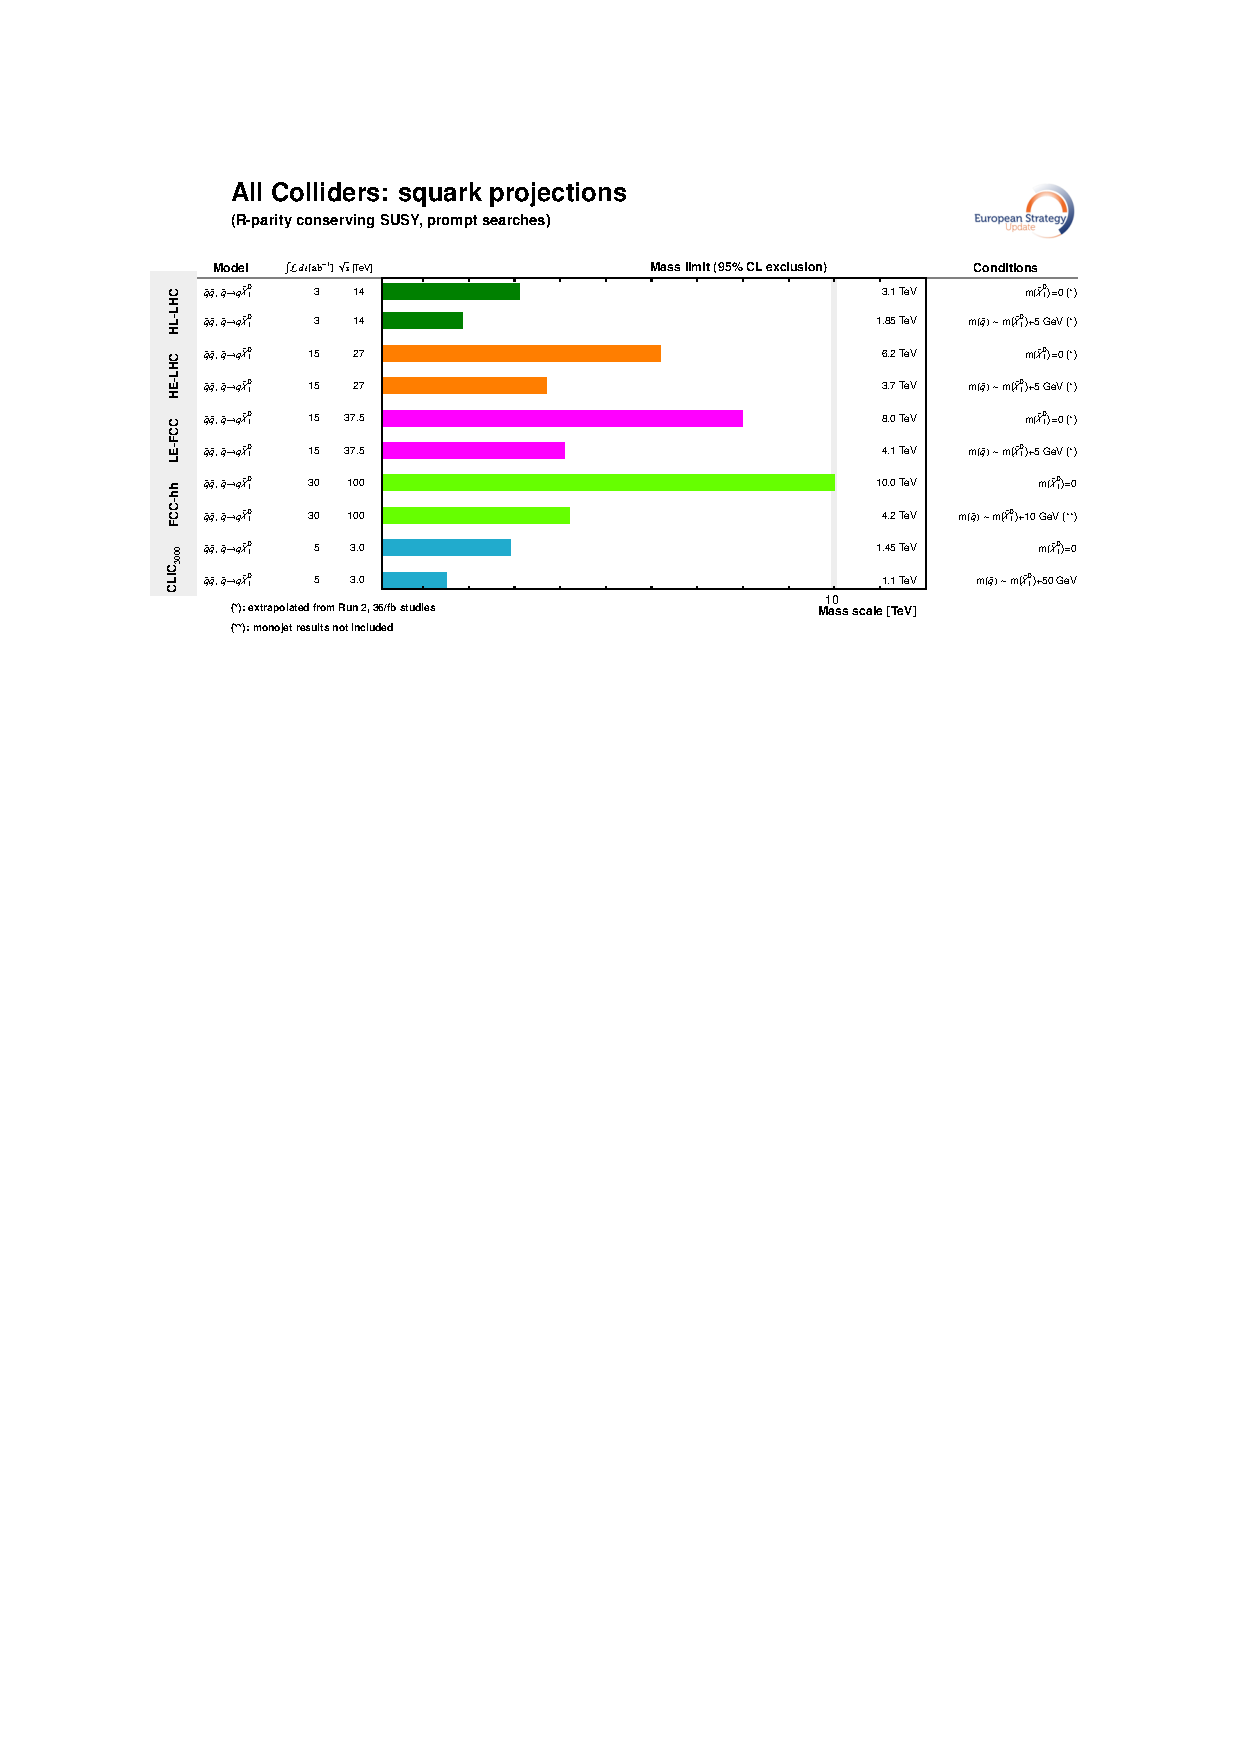
\includegraphics[width=1.0\textwidth]{\main/BSM/SUSY/plots_SUSY/AllCollider-Squark-cropped.pdf}
    \caption{
    Exclusion reach of different hadron and lepton colliders for first- and second-generation squarks.}
\label{fig:SUSY_squarks}
\end{figure}

Most studies of top squark (\tone) pair-production at hadron colliders assume $\tone \to t \chiOneZero$ and fully hadronic or semi-leptonic final states with large \Ptmiss. The best experimental sensitivity is achieved for 
$m(\chiOneZero ) \approx 0$ (i.e.~$\Dmstop \gg m_{t}$), while the reach in $m_{\tilde{t}}$~degrades for larger \chiOneZero~masses. For this reason, high-energy lepton colliders, e.g. \CLICThreeThousand,  might become competitive with \HLLHC in these topologies, as their stop mass reach is close to $\sqrt{s}/2$ even for low $\Dmstop$. Lower centre-of-mass energy lepton facilities do not have sufficient kinematic reach. The exclusion limits are summarised in Fig.~\ref{fig:SUSY_stop}; 
the discovery potential in all channels is about 5\% lower. If the \stopq$-$\chiOneZero~mass splitting is such that final states include very off-shell $W$ and $b$-jets, \stopq~masses up to about 1 TeV can be excluded at the \HLLHC~\cite{CidVidal:2018eel}. A two-fold and five-fold increase in reach is expected for the \HELHC~\cite{CidVidal:2018eel} and \FCChh~\cite{Abada:2019lih} respectively, with potential of improvements, especially in very compressed scenarios, via optimisation of monojet searches~\cite{Aaboud2018}.  

\begin{figure}[htb]
%\begin{figure}[t]
    \centering
%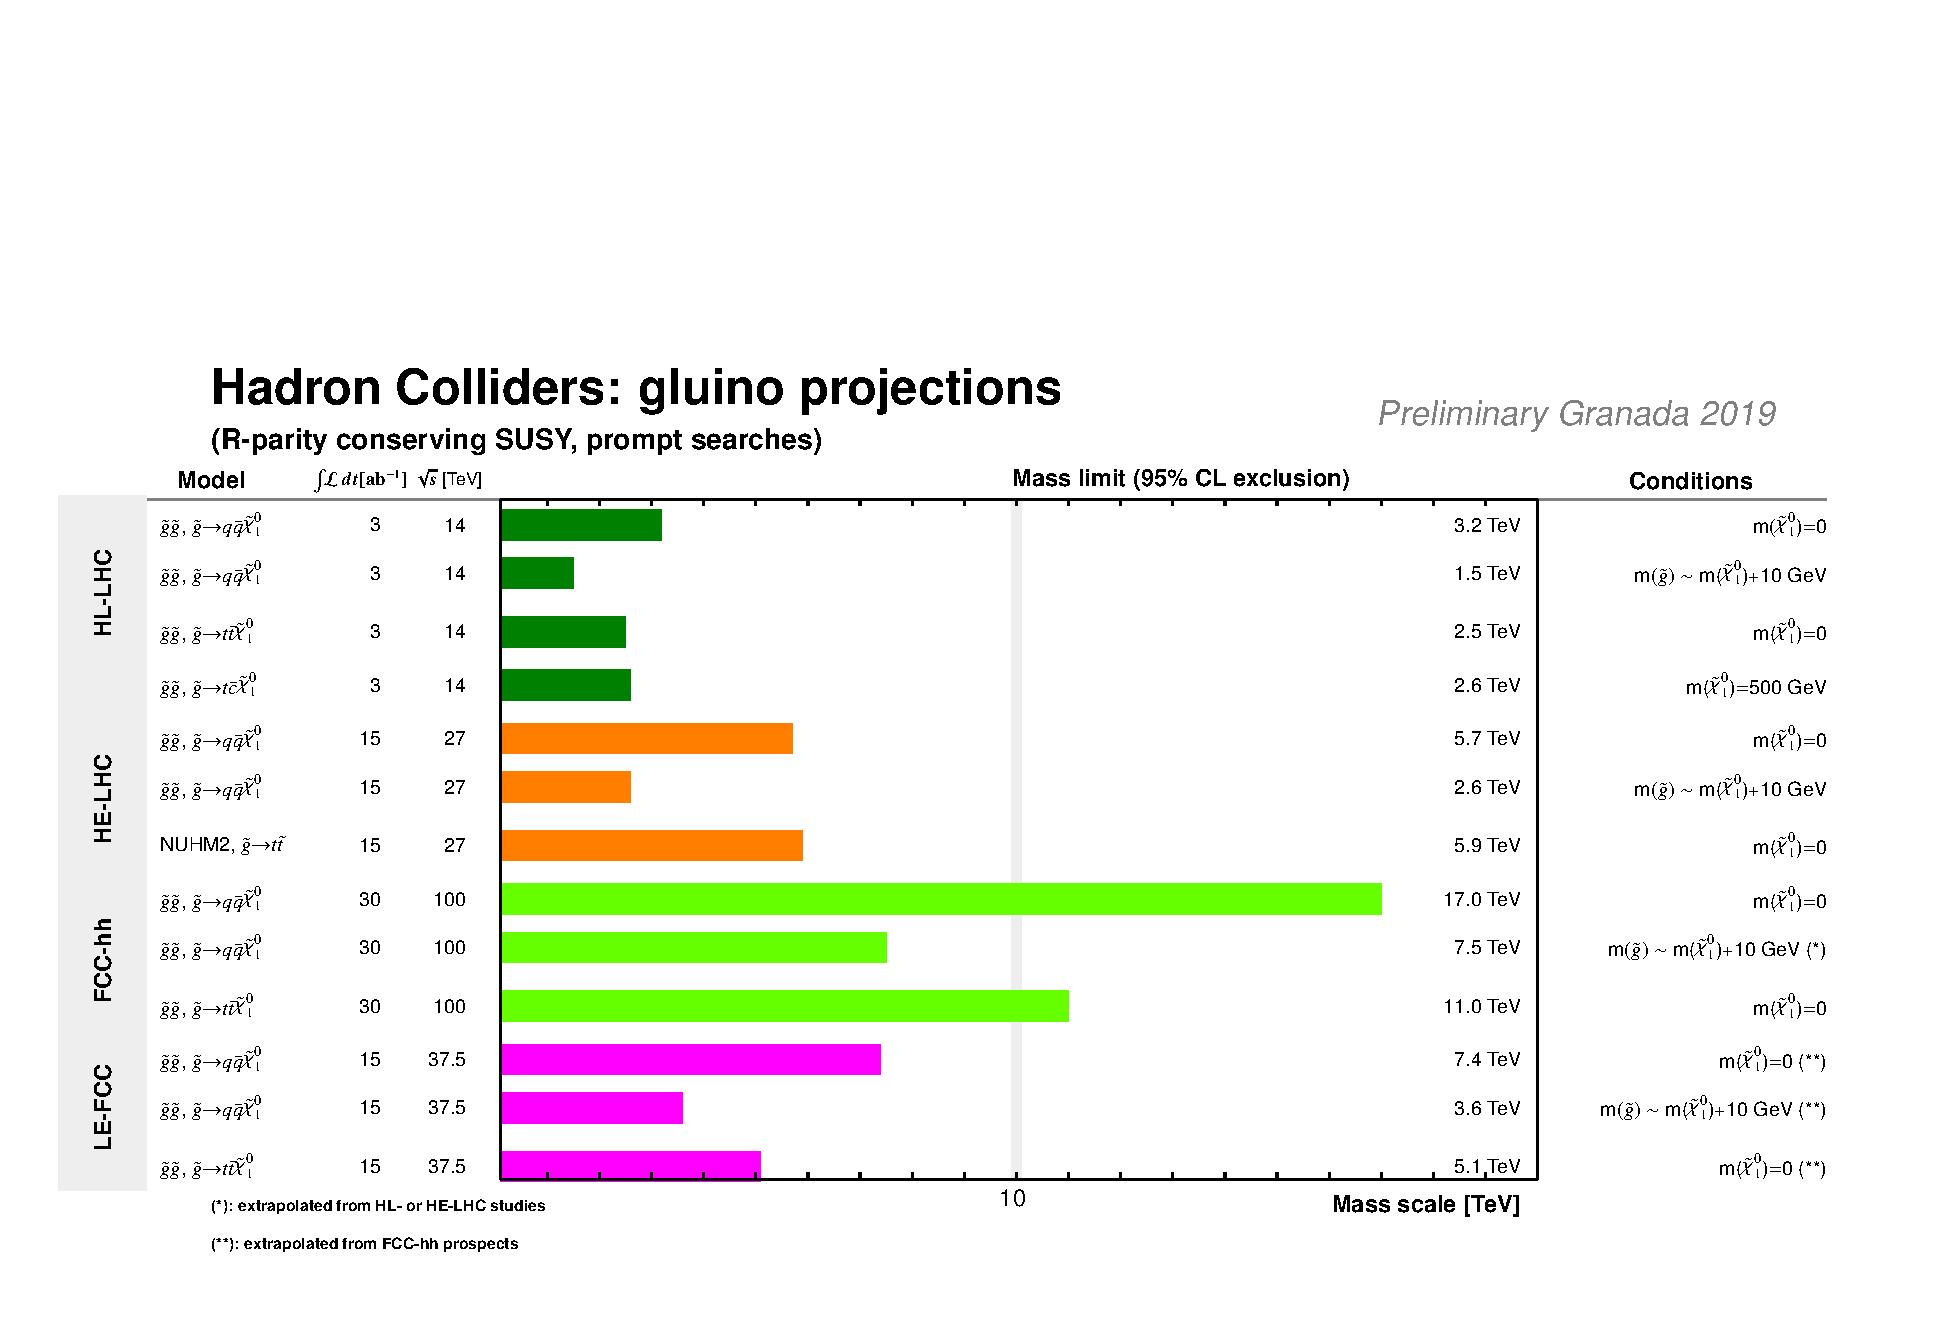
\includegraphics[width=0.45\textwidth]{\main/BSM/SUSY/plots_SUSY/AllCollider-Gluino-LEFCC.pdf}
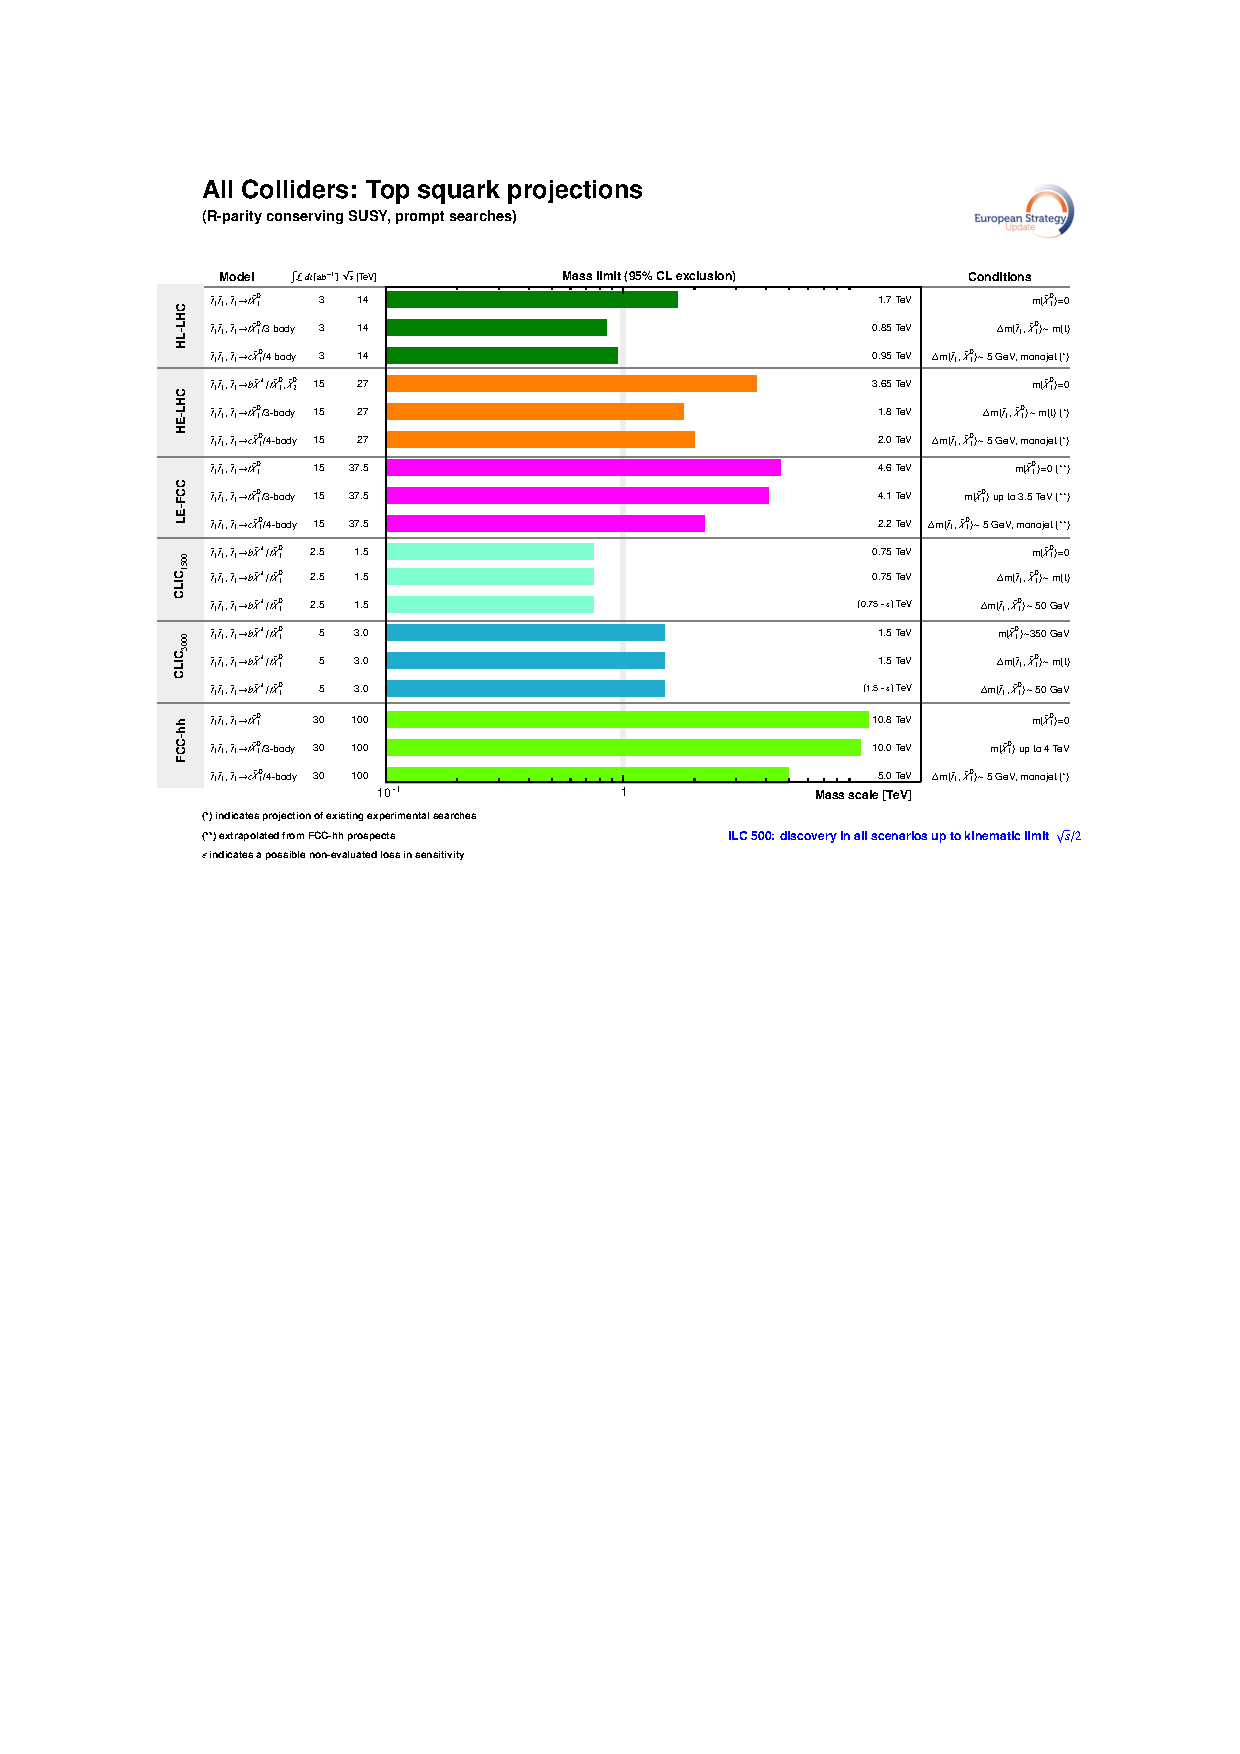
\includegraphics[width=1.0\textwidth]{\main/BSM/SUSY/plots_SUSY/AllCollider-Stop-LEFCC.pdf}
    \caption{
    %\emph{Left:} Exclusion reach for gluino pair production for hadron colliders \emph{Right:} 
    Top squark exclusion reach of different hadron and lepton colliders. All references are reported in the text. Results for CLIC have been communicated privately by the authors. Results for LE-FCC are extrapolated from HL- and HE-LHC studies. }
\label{fig:SUSY_stop}
\end{figure}


\begin{table}[t]
    \caption{Estimates of the degree of fine tuning in SUSY theories that can be probed with measurements of stop and gluino masses. The fine-tuning parameter is defined as $1/\epsilon \equiv \Delta m_h^2 / m_h^2$~\cite{Barbieri:1987fn}, where $\Delta m_h^2$ is the contribution to the physical Higgs mass $m_h$, which for stops (at one-loop) and gluino (at two-loops) is given by $1/\epsilon_{\tilde t}=(3y_t^2m_{\tilde t}^2/2\pi^2 m_h^2)\, \ln ({\Lambda }/ m_{\tilde t})$ and $1/\epsilon_{\gl}=(4y_t^2\alpha_s m_{\gl}^2/\pi^3 m_h^2)\, \ln^2 ({\Lambda }/ m_{\gl})$ in leading-log approximation. For high-scale SUSY-breaking mediation $\ln ({\Lambda }/ m_{\tilde t, \gl})\approx 30$ is taken, while for low-scale mediation $\ln ({\Lambda }/ m_{\tilde t, \gl})\approx 1$ is used.}
    \centering
               {\setlength{\extrarowheight}{14pt}
    \begin{tabular}{c||c|c}
       $\epsilon$  & High-scale mediation & Low-scale mediation \\
         \hline
         \hline 
         stop & $5\times 10^{-5} \left( \frac{\rm 10~TeV}{m_{\tilde t}}\right)^2$
           & $2\times 10^{-3} \left( \frac{\rm 10~TeV}{m_{\tilde t}}\right)^2$ \\
        gluino & $7\times 10^{-6} \left( \frac{\rm 17~TeV}{m_{\gl}}\right)^2$
           & $6\times 10^{-3} \left( \frac{\rm 17~TeV}{m_{\gl}}\right)^2$
    \end{tabular}}
    \label{tab:susyft}
\end{table}

Future collider searches of gluinos and stops will be powerful probes on the role of naturalness in the Higgs sector, as shown in Table~\ref{tab:susyft}. For a SUSY-breaking mediation mechanism near the unification scale, gluino searches at \FCChh will probe naturalness at the level of $10^{-5}$ and, even in the case of low-scale mediation, naturalness can be tested at the level of $10^{-3}$ from the leading stop contribution. 
Independently of any naturalness consideration, the measured value of the Higgs mass can be used as an indicator of the scale of SUSY particle masses. Indeed, in the minimal SUSY model, the prediction of the Higgs mass agrees with the experimental value only for stops in the multi-TeV range or larger. The most relevant range of stop masses can therefore be probed only at future hadron colliders. %since stops lighter than several TeV are inconsistent with the observed Higgs mass.

\subsection{Charginos, neutralinos and sleptons}
\label{sec:BSM-SUSY-weak}

In the context of $R$-parity conserving scenarios, the largest production rates for EWkinos in clean channels at hadron machines are obtained when the LSP is Bino-like and the lightest chargino (\chiOnePM) and next-to-lightest neutralino ($\tilde \chi_2^0$) are Wino-like, forming an approximately mass degenerate SU(2) triplet. 
Large $\tilde{\chi}_{2}^{0}\chiOnePM$ and $\chiOnePM\chiOneMP$ production rates and large mass splittings between the LSP and next-to-lightest SUSY states (NSLP) allow for the exploitation of multi-lepton final states at all facilities.
Figure~\ref{fig:SUSY_Winos} shows the exclusion reach for hadron and lepton colliders on the plane spanned by the relevant EWkino masses. For lepton colliders, the dominant processes are $e^+e^- \to$~\chiOnePM\chiOneMP, \chiTwoZero\chiOneZero; for hadron colliders only \chiTwoZero\chiOnePM ~production is considered here.
NLSP masses well above 1(2)~TeV could be reached by HL(HE)-LHC searches for a low-mass LSP~\cite{CidVidal:2018eel}; masses up to 3.3~TeV can be excluded at \FCChh~\cite{Golling:2016gvc}, with potential for improvements using optimised  selection criteria. Compressed SUSY spectra can be targeted at hadron colliders exploiting low-momentum leptons recoiling against an ISR jet. Lepton colliders analyses are competitive in this case: sensitivity up to EWkino masses equal to $\sqrt{s}/2$ are possible even for $\Delta m(\tilde{\chi}_{1}^{\pm}, \chi_1^0)$ as low as 1~\,GeV, with no loss in acceptance (ILC~\cite{Antusch:2017pkq}, CLIC~\cite{deBlas:2018mhx}).

\begin{figure}[htb]
%\begin{figure}[t]
    \centering
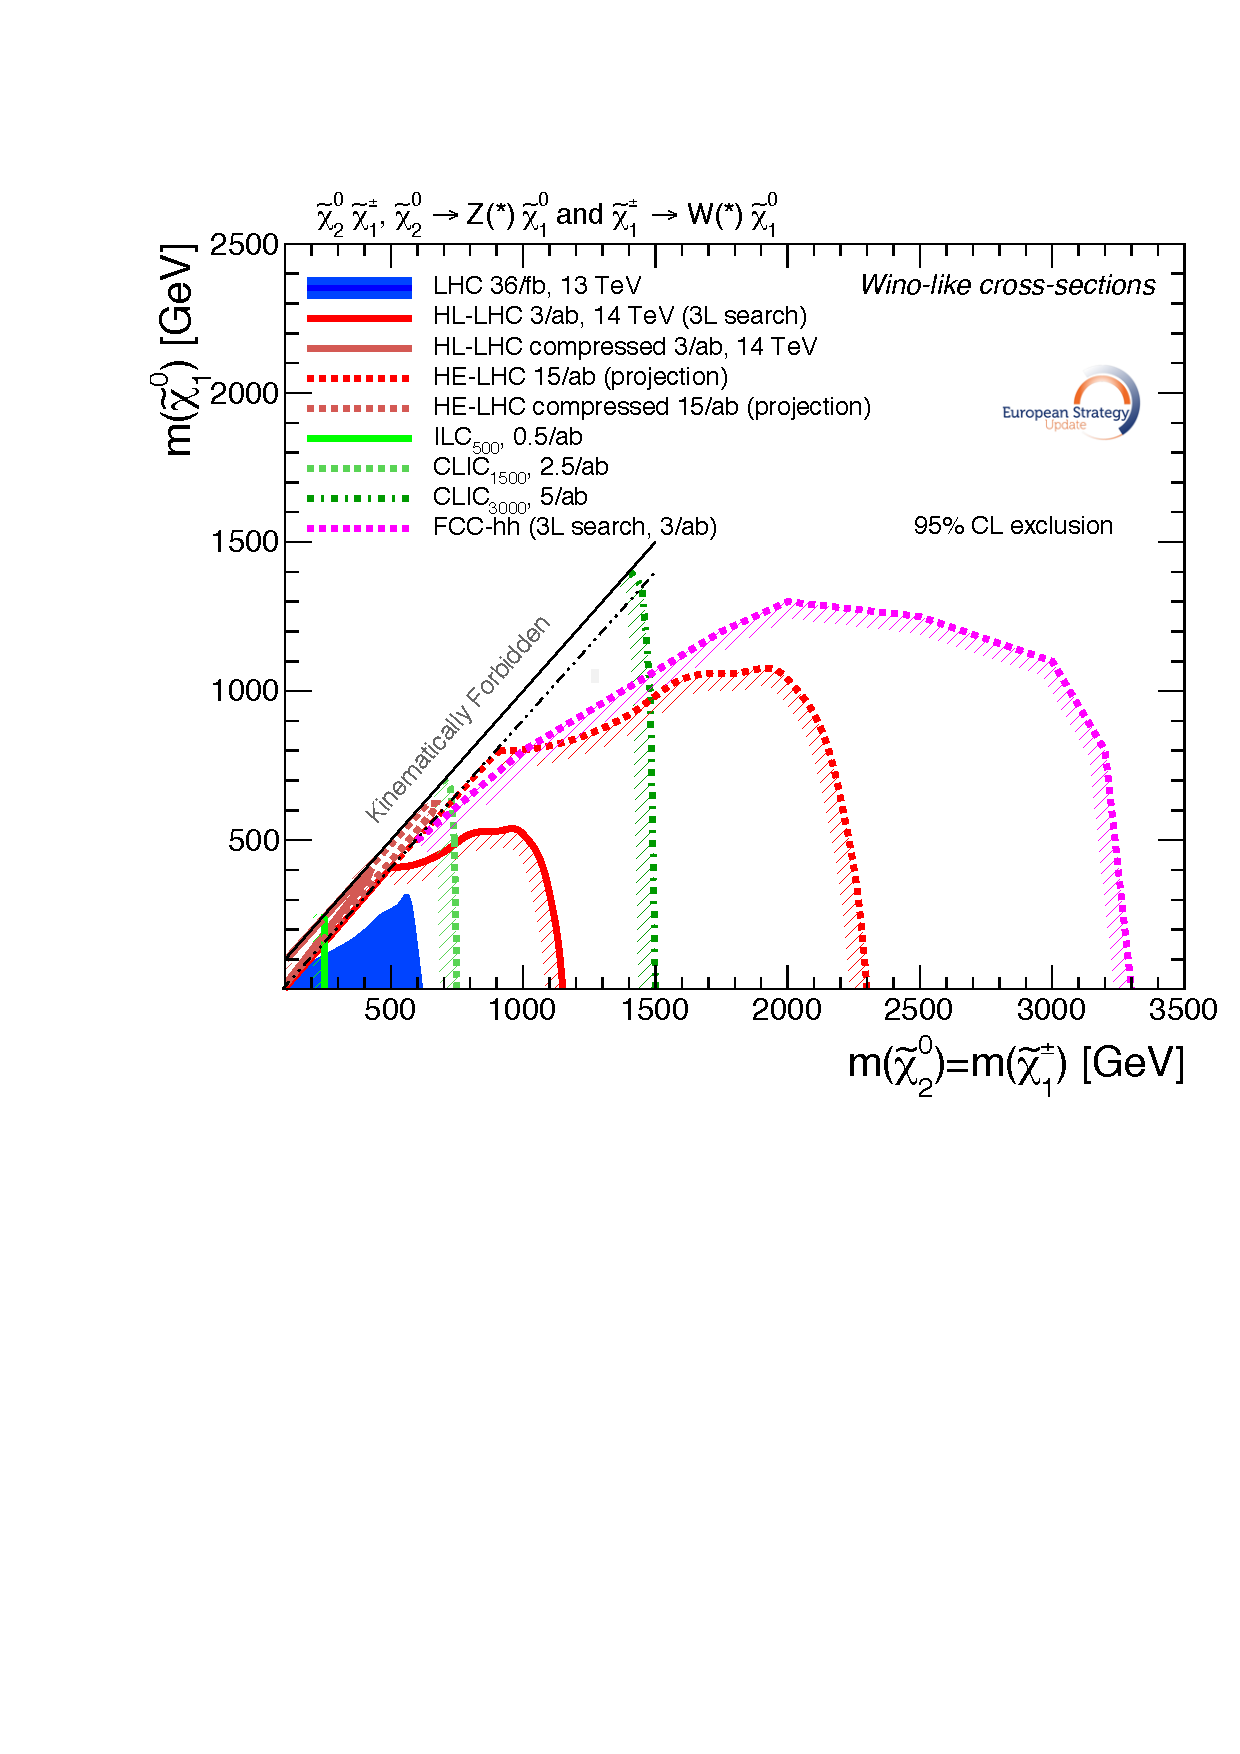
\includegraphics[width=0.7\textwidth]{\main/BSM/SUSY/plots_SUSY/C1N2_ES.pdf}
%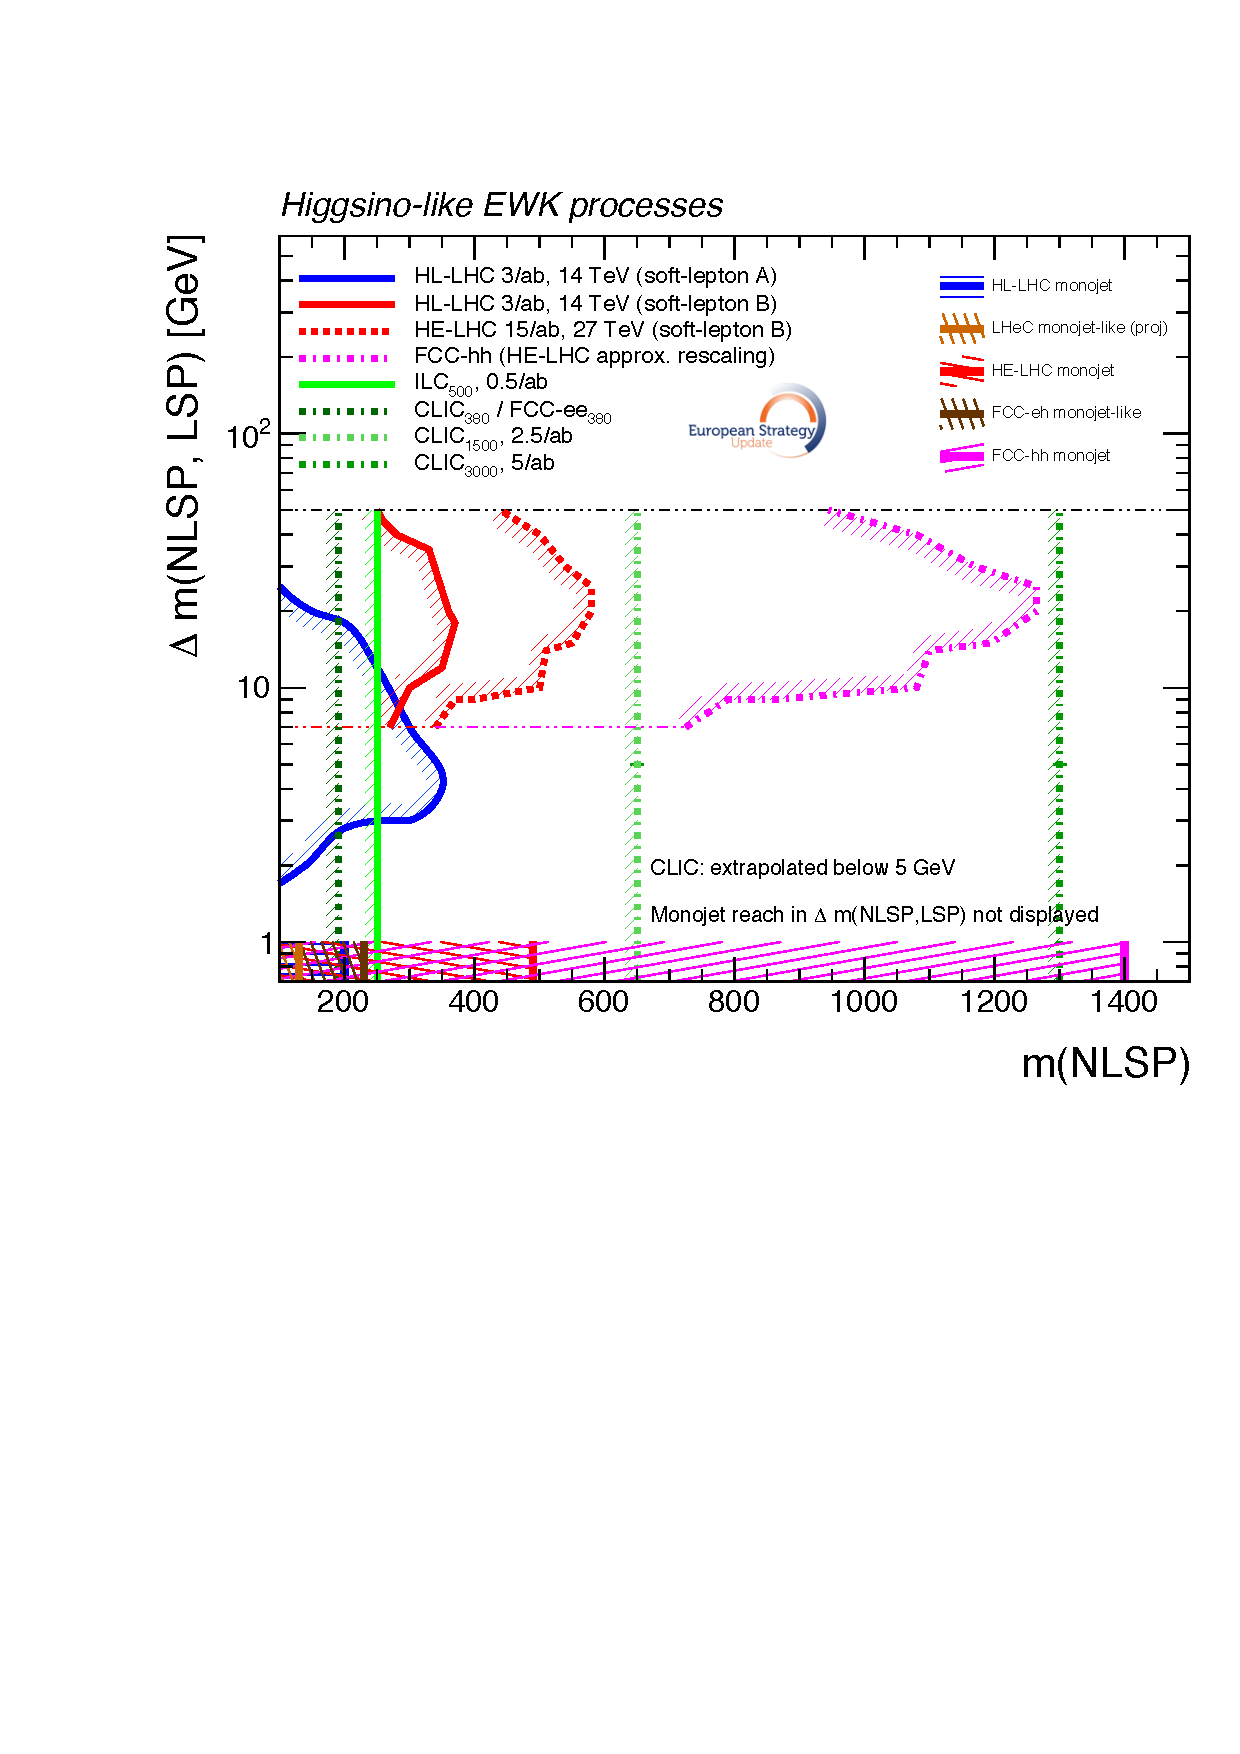
\includegraphics[width=0.8\textwidth]{\main/BSM/SUSY/plots_SUSY/DM_Higgsino_ES_withFCC.pdf}
    \caption{
    Exclusion reach for Wino-like lightest chargino (${\tilde \chi}_1^\pm$) and next-to-lightest neutralino (${\tilde \chi}_2^0$) from hadron and lepton colliders. %\emph{Right:} Exclusion reach for Higgsino-like charginos and next-to-lightest neutralinos where m($\tilde{\chi}_{1}^{\pm}$)$\sim$m($\tilde{\chi}_{2}^{0})=m$(NLSP), as a function of the $\Delta m$ between NLSP and LSP. Exclusion reaches using monojet searches at $pp$ and $ep$ colliders are also superimposed.}
    }
\label{fig:SUSY_Winos}
\end{figure}

If the Higgsino mass is much smaller than the gaugino masses, $\tilde \chi_{1,2}^0$ and \chiOnePM~form an approximately mass degenerate Dirac SU(2) doublet, and the EWkino spectrum is compressed. 
The EWkino production rates are smaller than in the previous case, making dedicated searches more challenging. Analyses exploiting ISR jets show good prospects at \HLLHC and hadron colliders in general (see Fig.~\ref{fig:SUSY_Higgsinos}):
\chiOnePM, \chiTwoZero~masses up to 350\,GeV can be probed at \HLLHC for mass splittings $\Delta m \equiv \Delta m (\tilde \chi_2^0,\tilde \chi_1^0 )\approx \Delta m (\tilde \chi_1^\pm,\tilde \chi_1^0 )$ between 0.8 and 50 GeV, 
with a factor 1.5 increase expected at the \HELHC~\cite{CidVidal:2018eel}. 
\FCChh projections computed with simple extrapolations show that the 1 TeV boundary might be reached, with expected 95\% CL limits up to 1.3~TeV depending on $\Delta m$.
On the other hand, the sensitivity of lepton colliders depend only weakly on the nature of the LSP: \ILCFiveHundred~\cite{Antusch:2017pkq} can cover the full mass range up to $\sqrt{s}/2$ for $\Delta m$ as low as 0.5~GeV, while CLIC$^{}_{1500}$ and \CLICThreeThousand allow a reach up to 650\,GeV and 1.3\,TeV, respectively (private communication).  
Monojet searches at hadron colliders can again complement the reach for scenarios with small $\Delta m$~\cite{CidVidal:2018eel}. The soft decay products of the NLSP are not reconstructed and the sensitivity solely depends on the production rate of EWkinos in association with an ISR jet. The reach of different colliders are illustrated by the hatched areas of Fig.~\ref{fig:SUSY_Higgsinos} for an indicative $\Delta m<1$~GeV. The sensitivity deteriorates at larger $\Delta m$, due to the requirements on additional leptons or jets. No attempt is made to evaluate this loss here, which is expected to become relevant for $\Delta m \approx 5$~GeV and above. Prospects for $ep$ colliders (LHeC and FCC-eh) performed using monojet-like signatures~\cite{Abada:2019lih} are also shown in Fig.~\ref{fig:SUSY_Higgsinos}.
%%% MD: original text 
%Monojet searches at hadron colliders can again complement the reach for scenarios with $\Delta m \approx 1$\,GeV, as reported in the hatched areas of Fig.~\ref{fig:SUSY_Higgsinos}. Prospects from $ep$ colliders (LHeC and FCC-eh) performed using monojet-like signatures are also shown for comparison.

\begin{figure}[htb]
%\begin{figure}[t]
    \centering
%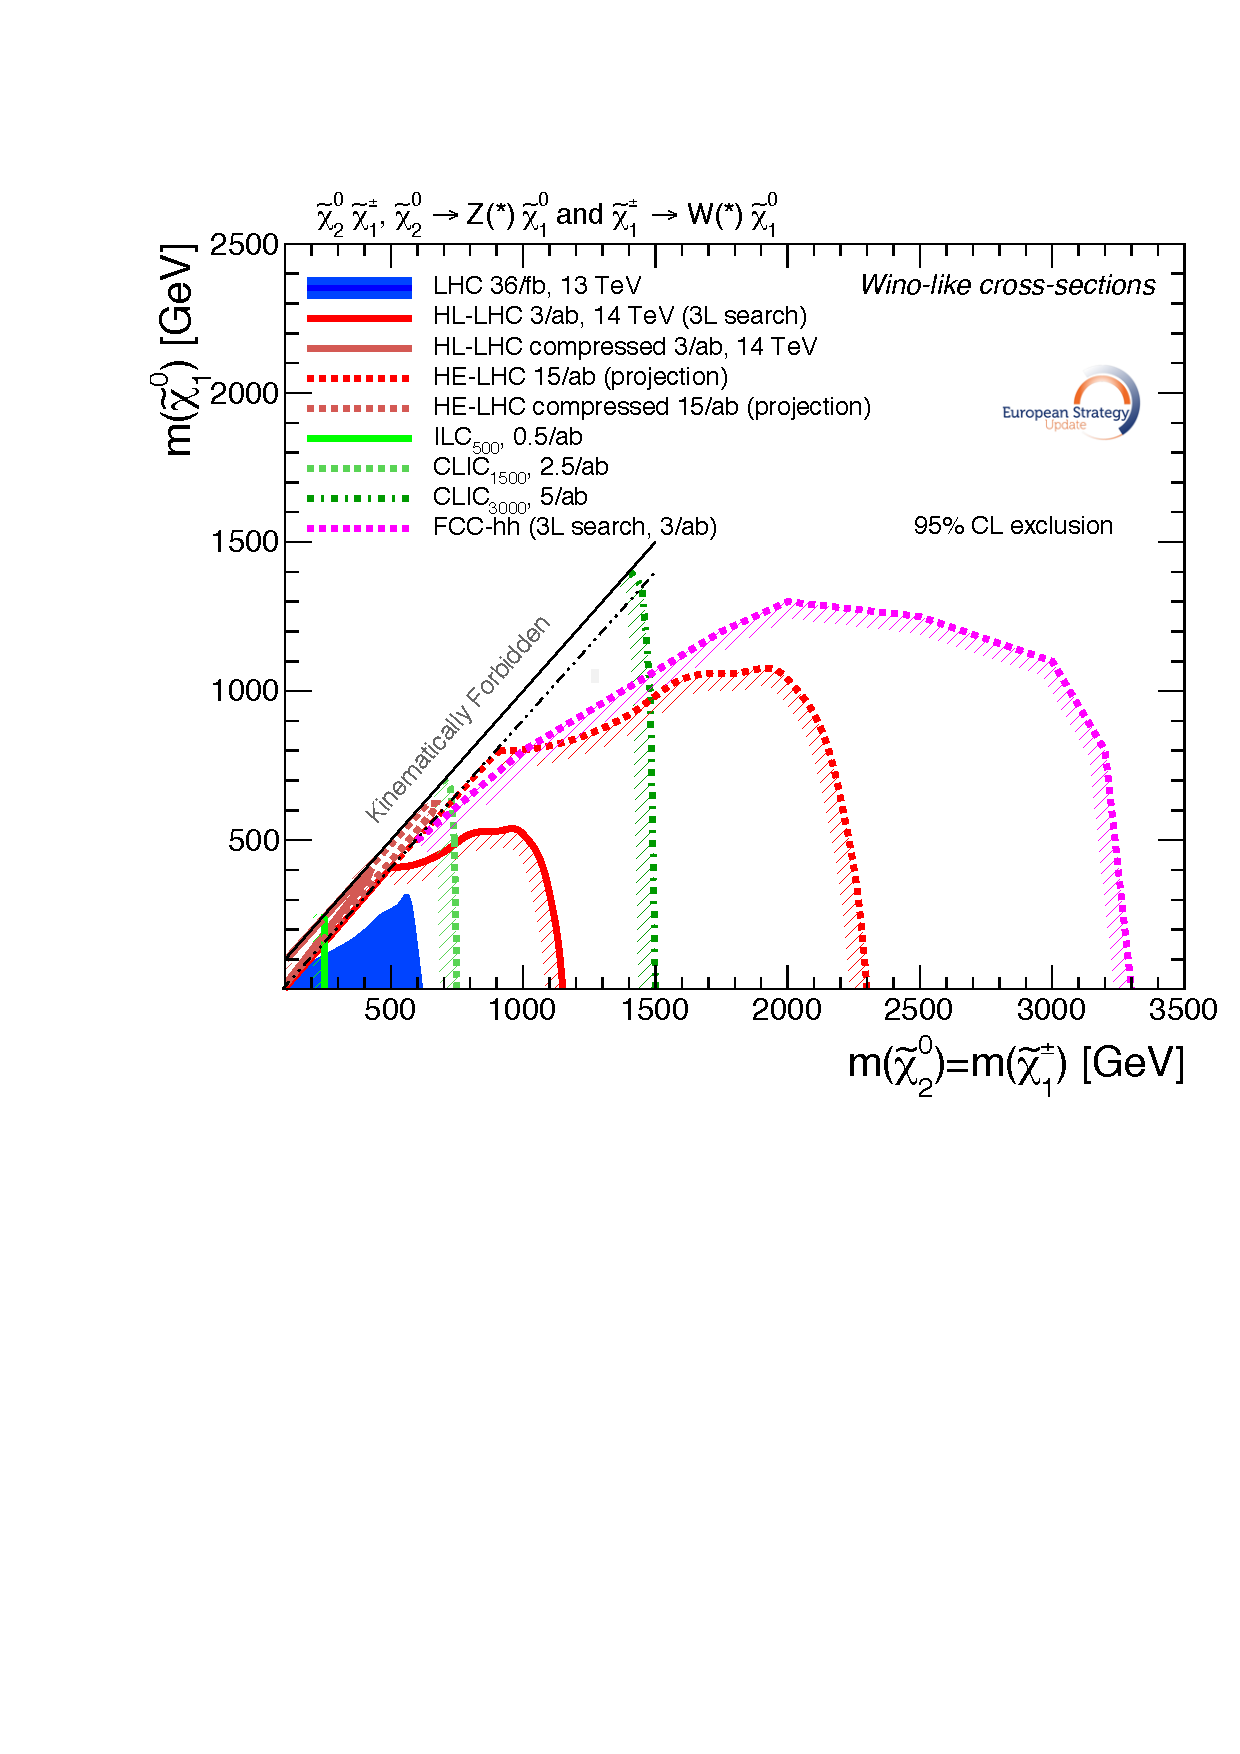
\includegraphics[width=0.45\textwidth]{\main/BSM/SUSY/plots_SUSY/C1N2_ES.pdf}
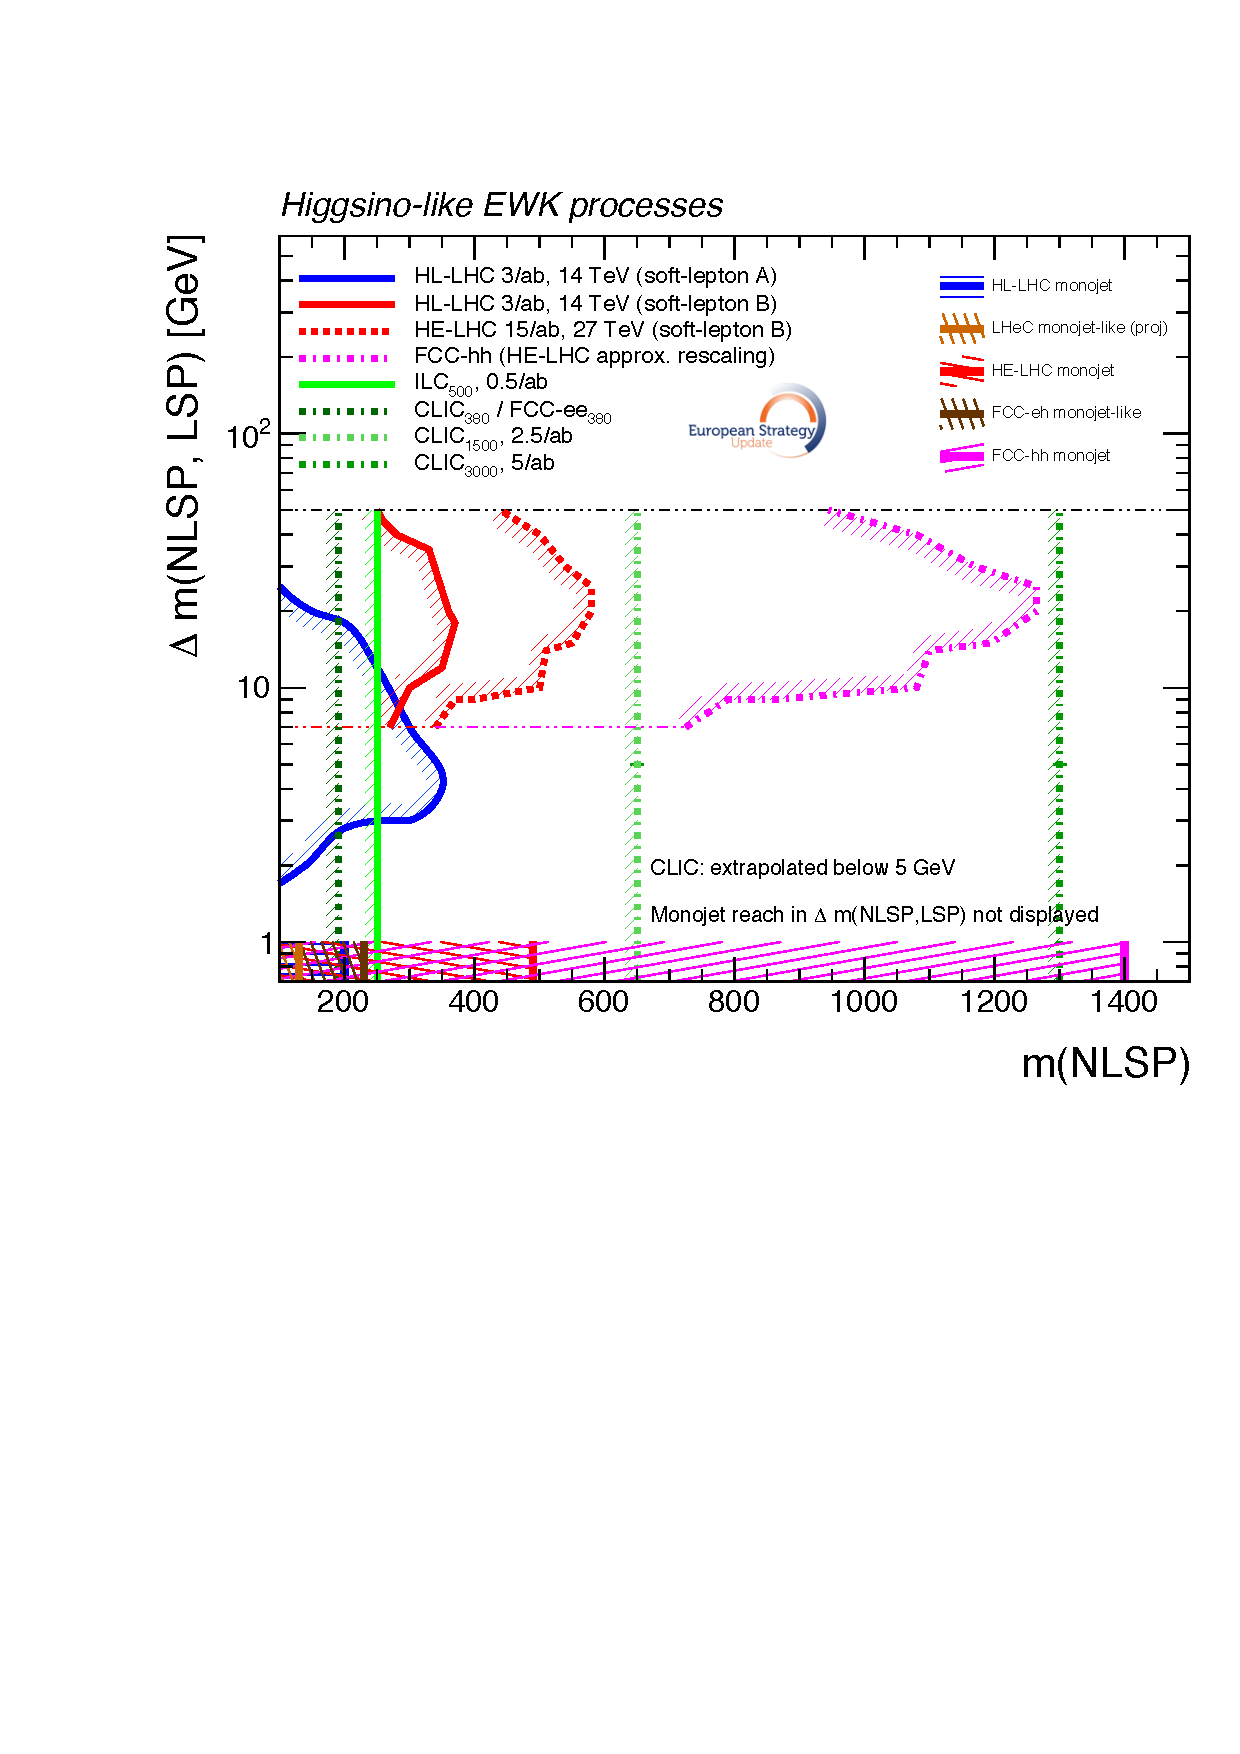
\includegraphics[width=0.7\textwidth]{\main/BSM/SUSY/plots_SUSY/DM_Higgsino_ES_withFCC.pdf}
    \caption{
    %\emph{Left:} Exclusion reach for lightest chargino and next-to-lightest neutralino production for hadron and lepton colliders, for Wino-like states. Contours are shown for \HLLHC, \HELHC, \FCChh as well as \ILCFiveHundred, CLIC$^{}_{1500}$ and \CLICThreeThousand. 
    Exclusion reach for Higgsino-like charginos and next-to-lightest neutralinos with equal mass $m\,$(NLSP), as a function of the mass difference $\Delta m$ between NLSP and LSP. Exclusion reaches using monojet searches at $pp$ and $ep$ colliders are also superimposed (see text for details).}
\label{fig:SUSY_Higgsinos}
\end{figure}
%%%%%%%%%%% 
% MD: rephrased: It has been simplified to ensure there isn't confusion between the reaches given for disappearing tracks analysis here - simplified models - and in the dark matter section (fig 13), but also to improve the legacy between the two sections.  
%%%%%%%%%%%
A special case arises when the lightest neutralino is either pure Higgsino or Wino. The chargino-neutralino mass splitting is around 340 MeV and 160 MeV respectively, and the chargino has a correspondingly long lifetime. The value of \Ptmiss~is small unless the pair-produced EWkinos recoil against an ISR jet. Taking advantage of the long lifetime of the charginos, searches for disappearing charged tracks can be performed at hadron colliders. As an example, at the \HLLHC, studies using simplified models of \chiOnePM~production lead to exclusions of chargino masses up to $m_{{\tilde \chi}_1^\pm}$ = 750\,GeV (1100\,GeV) for lifetimes of 1\,ns for the Higgsino (Wino) hypothesis. When considering the lifetimes corresponding to the chargino-neutralino mass splittings given above (leading to thermal relic dark matter candidates and referred to as pure Higgsino and pure Wino, respectively), masses up to 300 (830)~GeV can be excluded. The reach for all facilities is illustrated in Sect.~\ref{sec:BSM-DM}. Analyses exploiting displaced decays of the charged SUSY state have been studied also for lepton colliders, e.g.\ \CLICThreeThousand (using charge stub tracks~\cite{deBlas:2018mhx}), and for $ep$ colliders (using disappearing tracks~\cite{Curtin2018}).  

%%%%%%%%%%%%%
% MD: below is the original version.  
%%%%%%%%%%%%%
% A special case arises when the lightest neutralino is either pure Higgsino or Wino. The chargino-neutralino mass splitting is around 340 MeV and 160 MeV respectively, and the chargino has a correspondingly long lifetime. The value of\Ptmiss~is small unless the pair-produced EWkinos recoil against an ISR jet. Taking advantage of the long lifetime of the charginos, searches for disappearing charged tracks can be performed. At the \HLLHC, studies using simplified models of \chiOnePM~production lead to exclusions of chargino masses up to m(\chiOnePM) = 750\,GeV (1100\,GeV) for lifetimes of 1\,ns for the Higgsino (Wino) hypothesis.  When considering the lifetimes corresponding to the chargino-neutralino mass splittings given above, masses up to 300 (830)~GeV can be excluded.  Assuming a detector similar to those  available for \HLLHC, at the \HELHC Winos (Higgsinos) can be discovered for masses up to 1500 (450) GeV.  An up to three-fold increase is expected at the \FCChh, and access to thermal relic dark matter candidates will be possible (see Sect.~\ref{sec:BSM-DM}). Analyses exploiting displaced decays of the charged SUSY state and/or disappearing track signatures have been performed also for \CLICThreeThousand and for $ep$ colliders. 
% MD: slightly modified to better define the CLIC approach. 
 
Collider experiments have significant sensitivity also to sleptons. Searches for staus, superpartners of $\tau$ leptons, might be particularly challenging at $pp$ facilities due to the complexity of identifying hadronically-decaying taus and reject misidentified candidates. Analysis of events characterised by the presence of at least one hadronically-decaying $\tau$ and \Ptmiss~show that the \HLLHC will be sensitive to currently unconstrained pair-produced $\tilde{\tau}$ with discovery (exclusion) potential for $m_{\tilde{\tau}}$ up to around 550~(800)~GeV~\cite{CidVidal:2018eel}. The \HELHC would provide sensitivity up to 1.1~TeV~\cite{CidVidal:2018eel}, and an additional three-fold increase is expected for the \FCChh (extrapolation). 
Lepton colliders could again provide complementary sensitivity especially in compressed scenarios: \ILCFiveHundred~\cite{Antusch:2017pkq} would allow discovery of $\tilde{\tau}$ up to 230~GeV even with small datasets, whilst  \CLICThreeThousand would allow reach up to $m_{\tilde{\tau}}=1.25$~TeV and $\Delta m(\tilde{\tau},\chi_1^0)=50$~GeV (private communication). 

\subsection{Non-prompt SUSY particles decays}
There are numerous examples of SUSY models where new particles can be long-lived and may travel macroscopic distances before decaying. Long lifetimes may be due to small mass splittings, as in the case of pure Higgsino/Wino scenarios, or due to small couplings, as in $R$-parity violating SUSY models, or due to heavy mediators, as in Split SUSY.
For \HLLHC~\cite{CidVidal:2018eel}, studies are available on long-lived gluinos and sleptons. Exclusion limits on gluinos with lifetimes $\tau>0.1$\,ns can reach about 3.5 TeV, using reconstructed massive displaced vertices. Muons displaced from the interaction point, such as found in SUSY models with $\tilde{\mu}$ lifetimes of $c\tau > 25$ cm, can be excluded at 95\% CL at the \HLLHC. New fast timing detectors will also be sensitive to displaced photon signatures arising from long-lived particles in the $0.1 < c\tau < 300$ cm range.

Complementarities in long-lived particle searches and enhancements in sensitivity might be achieved if new proposals for detectors and experiments such as MATHUSLA200, FASER, CODEX-b, MilliQan and LHeC are realised in parallel to the HL-LHC. As an example, with a zero-background hypothesis, MATHUSLA200~\cite{Curtin:2018mvb} would offer a coverage complementary to \HLLHC in terms of new particles with $c\tau$ in the range 100~m -- 20~km, targeting $R$-parity violating decays of gluinos, top squarks as well as sleptons and Higgsinos.

\end{document}

